\section{Evaluation}
\label{sec:evaluation}

In this section we present the results of evaluating the energy-saving effects
of using a block-level solution on a SAN environment. There are two
configurations that are compared; the first is the baseline case where a client
machine accesses its back-end storage through an iSCSI connection to a remoter
storage server. In this case, both client and server machines are utilized when
I/O is performed. The client's memory capacity will determine the amount of data
that is cached from the server-side and thus the amount of interactions with the
server. As for the DM-Cache setup, an SSD is used an as additional cache layer
between the client and the server. This layer provides a larger capacity to
cache more data from the server-side, and thus reduce interactions with it. Two
kinds of configurations of DM-Cache are tested; one that caches data from read
operations but sends writes directly to the source device, and one configuration
that caches data from both read and write operations.

\subsection{Experimental Setup}

These tests were performed on two nodes that are part of a Dell 2970
cluster. The source device and the cache device were in separate servers, which
are running Linux 2.6.32 on Ubuntu with 24 GB of RAM.  The initiator (client) is
connected to the target device (source device) using the iSCSI protocol. The
initiator server contained the two disks, an HDD that was used as local storage,
and an SSD that was used as the cache device. The HDD was a 1 TB Seagate
Constellation ES 7200 RPM disk. The SSD cache was a 120 GB Intel SSD 320
Series. The target server (storage server) contained four 1TB HDD with
specifications similar to the one used in the initiator server. One of these was
used for local storage, and another was used as the source device. The remaining
two were not used as part of the tests. For every test DM-Cache was configured
to use a block size of 8 sectors, an associativity of 256, and a cache size of
64 GB. As for the benchmarking tool, IOzone 3.398 was used. All I/O operations
were done on a file of size of 8GB or 12GB, and with a request size of 4 KB.

\subsection{Measuring Power Consumption}

In order to measure the power consumption of a node we used the Watts up? PRO
power meter \cite{wattsup}. This power meter measures the power consumption in
watts with an interval as fast as one second. It came with a USB cable adapter
which we used in combination with an open-source Linux utility tool in order to
download the data directly to a PC.

\subsection{Workloads}

There are several workloads that can receive potential power consumption saving
from using client-side caching. Specifically, clients will benefit more when the
workloads access data that has already been cached to the client-side SSD
device. A system that uses DM-Cache with write-back configuration can support
operations like these. For example, write and read operations which produce hits
on the cache will reduce load on the server-side storage device, and at the same
time reduce the amount of power consumed on the storage server. For the baseline
system setup, a read may be served from the system’s page cache, but writes will
always have to be dispatched to the storage server. This results in a constant
use of the server storage device.

Because of the nature of a cache device, we also consider the effect of cache
misses on power consumption. Cache misses caused by operations like a cold read
will inevitably have greater power consumption than the current iSCSI
system. This is because they result in a read operation to read data from the
server storage, and a write operation to write data on the client-side SSD
cache. Thus, workloads that have greater cache hit ratios are the most
appropriate for this type of system.

\subsection{Energy Consumption Results}

\begin{table}
  \centering
  \resizebox{\linewidth}{!}
  {
    \begin{tabular}{|l|l|l|l|l|}
      \hline & \bf iSCSI-W & \bf DMC-WT & \bf DMC-WB-M & \bf DMC-WB-H \\ \hline
      Client & 15589.3     & 16035.6    & 13316.2      & 11664.2      \\ \hline
      Server & 17754.7     & 17874.1    & 14479.4      & 13170.5      \\ \hline
      Total  & 33344       & 33909.7    & 27795.6      & 24834.7      \\ \hline
    \end{tabular}
  }
  \caption{Energy consumption (in Joules) of write operations using an 8GB file}
  \label{tab:write-energy}
\end{table}

\begin{table}
  \centering
  \resizebox{\linewidth}{!}
  {
    \begin{tabular}{|l|l|l|l|}
      \hline & \bf iSCSI-R & \bf DMC-R-M & \bf DMC-R-H \\ \hline
      Client & 13168.8     & 16163.8     & 9119.3      \\ \hline
      Server & 15189       & 18068.1     & 10363.8     \\ \hline
      Total  & 28537.8     & 34231.9     & 19483.1     \\ \hline
    \end{tabular}
  }
  \caption{Energy consumption (in Joules) of read operations using an 8GB file}
  \label{tab:read-energy}
\end{table}

In order to get a general idea of the difference between the power consumption
of I/O requests which are served from the cache device, and those that are
served from the storage server, we performed simple sequential I/O operations
using a tool like IOzone. Table ~\ref{tab:write-energy} shows the energy
consumption of both the client and server machines when performing write
requests. The second column (iSCSI-W) shows the energy consumption of writes
performed on with the plain iSCSI system setup. This is the value that we'll use
as a baseline to compare the energy consumption of a system running with
DM-Cache. The next column shows the energy consumption of writes performed on a
system the write-through configuration of DM-Cache (DMC-WT).  Because
write-through operations on DM-Cache are similar to regular iSCSI writes, the
difference between energy consumption of these two is not too much.  The shows
fourth column, a write-back miss (DMC-WB-M), shows energy power consumption of
doing writes on a file that has not been yet cached. Even though this operation
involves cache misses, the energy consumption for this operation is less than
the previous tests, because there are very few reads performed on the server
storage in comparison the number of writes done on the SSD. The last operation
involves writes that produce cache hits. These are the fastest and also the most
energy efficient of all operations.

Table ~\ref{tab:read-energy} shows the energy consumption of sequential read
requests. The second columns shows the energy consumed by reads performed on the
system without DM-Cache. The next column shows the results of read misses using
DM-Cache. The results in this particular category show the additional energy
consumed when a read causes a cache miss. The additional energy is caused by the
fact that both the client and server are actively performing I/O, and also
because of the length of the operation. The last column shows the energy saving
potential of client-side caching, as a read hit operation shows a significant
reduction in energy consumption.

Results confirm previous expectations that an SSD cache can help reduce power
consumption. For operations where I/O's are served from the cache device, SSD's
can save up to 25\% energy savings for write operations, and 32\% for read
operations.

\subsection{Analysis}

\begin{figure}[t]
  \caption{Power consumption of write operations on the client}
  \centering 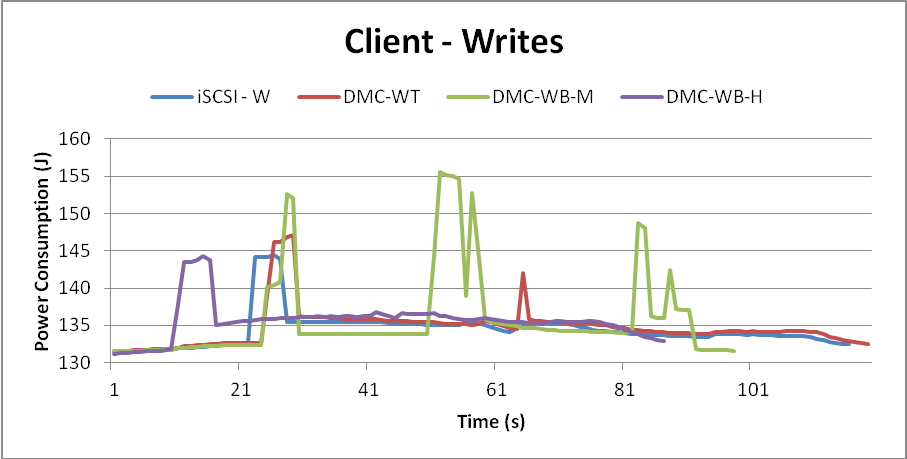
\includegraphics[width=\linewidth]{client_writes.png}
  \label{fig:client-writes}
\end{figure}

\begin{figure}[t]
  \caption{Power consumption of write operations on the server}
  \centering 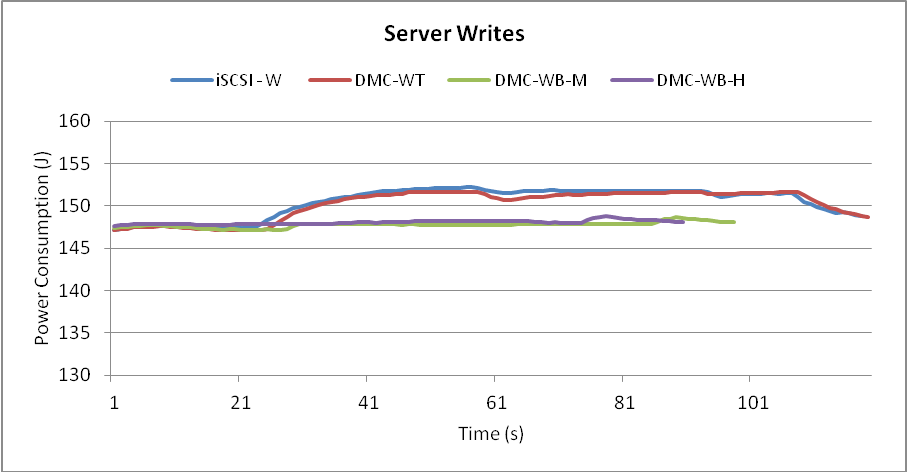
\includegraphics[width=\linewidth]{server_writes.png}
  \label{fig:server-writes}
\end{figure}

\begin{figure}[t]
  \caption{Power consumption of read operations on the client}
  \centering 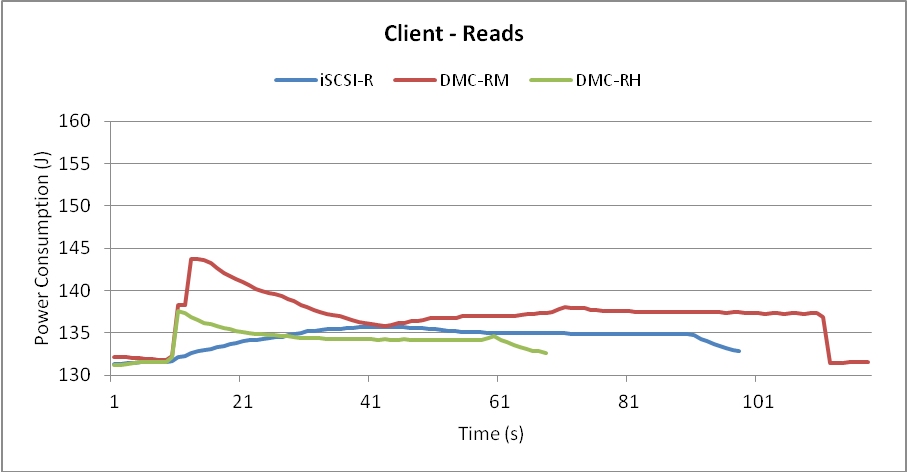
\includegraphics[width=\linewidth]{client_reads.png}
  \label{fig:client-reads}
\end{figure}

\begin{figure}[t]
  \caption{Power consumption of read operations on the server}
  \centering 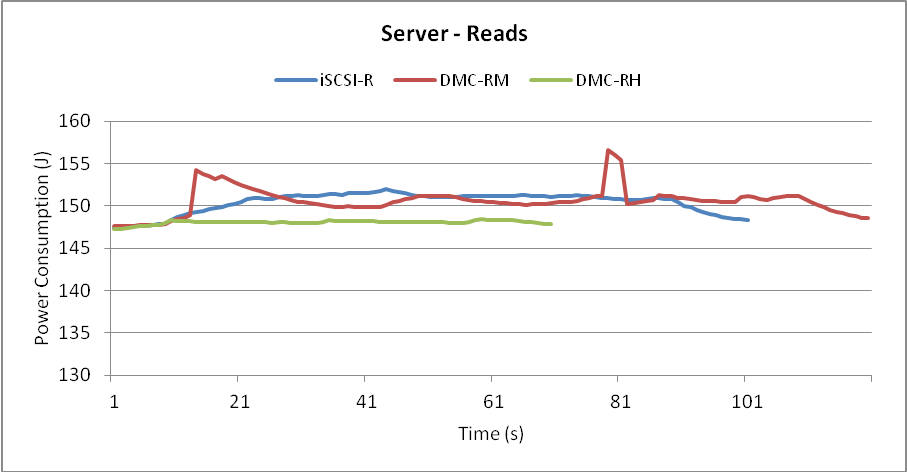
\includegraphics[width=\linewidth]{server_reads.png}
  \label{fig:server-reads}
\end{figure}

In this section we explore the reasons behind the results of the energy
consumption benefits obtained from an SSD client-side cache device. In order to
this we observe the power consumption graphs yielded by each operation. These
graphs give us several perspectives of the operation ranging from the execution
time of the operation to the power consumption of a specific point in
time. Firstly, let's observe the sequential write operation using the
write-through configuration of DM-Cache. This DM-Cache operation is equivalent
to the regular iSCSI because only reads are served from the cache device, but
write requests are left to be directed to the source device as they normally
would. This means that it is expected that the performance of the iSCSI-W and
the DMC-WT operations be the same or close. Either Figure
~\ref{fig:client-writes} or Figure ~\ref{fig:server-writes} can be checked to
confirm that the execution time for these two operations is close, therefore
translating to a similar throughput. A slight increase in power consumption is
seen on the client-side but very little difference on the server-side. The next
test shows the power consumption of DMC-WB-M, which is a write operation that
results in cache misses when performed on the write-back configuration of
DM-Cache. Figure ~\ref{fig:client-writes} shows that this operation contains
several spikes of high power consumption on the client-side machine. The reason
for which this operation consumes less energy than an iSCSI-W is that this
operation takes less time to execute and also the power consumption on the
server-side is significantly lower than its corresponding iSCSI-W operation. The
last test is DMC-WB-H, which represents a write operation that results in mostly
cache hits on a write-back configuration of DM-Cache. This operation has a low
power consumption rate on both the client and server-side, and also has a much
faster execution time. This results in the operation that consumes the least
amount of energy.

Figure ~\ref{fig:client-reads} and Figure ~\ref{fig:server-reads} show the power
consumption of reads on the client and the server side, respectively. The
operation DMC-RM are the reads that are performed on the write-back
configuration of dm-cache that are done on data that is not on the cache device
and result on cache misses. This operation consumes around 18\% more energy than
the iSCSI-R operation. The reason is because a read cache miss triggers a fetch
operation to bring in the data from the source device and another operation to
store this data on the SSD cache device. These additional I/O requests result in
a slower throughput and more energy consumption on both client and server-side,
in comparison to the baseline iSCSI-R operation.  The other read operation,
DMC-RH, shows the power consumption cause by read cache hits. Figure
~\ref{fig:server-reads} shows that initially the power consumption of this
operation on the client-side is similar or slightly higher than the iSCSI-R
operations; however, because of its shorter execution time the operation results
in lower energy consumption. On the server-side power consumption remains low
because the HDD source device remains idle since all read requests are served
from the cache device.
